% Created 2025-10-02 Thu 02:42
% Intended LaTeX compiler: pdflatex
\documentclass[11pt]{article}
\usepackage[utf8]{inputenc}
\usepackage[T1]{fontenc}
\usepackage{graphicx}
\usepackage{longtable}
\usepackage{wrapfig}
\usepackage{rotating}
\usepackage[normalem]{ulem}
\usepackage{amsmath}
\usepackage{amssymb}
\usepackage{capt-of}
\usepackage{hyperref}
\author{grupert}
\date{\today}
\title{Diretoria-App Documentation}
\hypersetup{
 pdfauthor={grupert},
 pdftitle={Diretoria-App Documentation},
 pdfkeywords={},
 pdfsubject={},
 pdfcreator={Emacs 30.2 (Org mode 9.7.11)}, 
 pdflang={English}}
\begin{document}

\maketitle
\tableofcontents

\section{Diretoria-App}
\label{sec:org5556508}
\subsection{1. Introdução}
\label{sec:org7a4c75a}
Desenvolvimento de um sistema que siga as práticas normativas de Engenharia de Software em um projeto que modela e organiza nossas atividades em um lugar centralizado.
Além de seguir as bases teóricas de bancos de dados, engenharia de software, e uma metodologia ágil no desenvolvimento, precisamos que a aplicação tenha uma interface gráfica responsiva e intuitiva, que garanta que todos os moradores possam utilizar a aplicação web.
O sistema armazenará dados sobre as atividades da república em diferentes áreas - inicialmente - a venda de salgados na faculdade, um gerenciamento básico de usuário, o controle de produtos, e a submissão de manutenções necessárias na casa.
\subsection{2. Visão Geral da Aplicação}
\label{sec:orga6c0ba0}
O site será composto por uma tela de login/cadastro, que direcionará o usuário a uma página com um calendário, e cards que direcionam o usuário para: salgados, pedido de manutenção, e um controle de produtos. 
\subsubsection{2.1 Calendário}
\label{sec:org43feda5}
O calendário será apresentado visualmente usando javascript, e usará os dados contidos no banco de dados para diferentes visualizações. Um usuário ativo, membro da área \uline{X} deve ser capaz de visualizar todos os eventos pertencentes à sua área, e da área \uline{geral}, uma área especial criada para que possamos compartilhar informações e datas pertinentes a todos.
Posteriormente, um usuário deve ser capaz de adicionar eventos e removê-los, selecionado a qual área o evento pertence.
\subsubsection{2.2 Pedido de manutenção}
\label{sec:org5b21fbc}
Um usuário poderá fazer o upload de uma foto e uma descrição, associados a um cômodo da república e ao morador que fez o envio. Todos os envios neste formulário serão visíveis para membros da área \uline{responsavel\textsubscript{manutencao}}, moradores do quarto afetado (se aplicável), e o responsável pelo envio do pedido. Todos esses deverão ser capazes de ver o status da manutenção (definido pelo responsável pela manutenção), e as outras informações do pedido.
\subsubsection{2.3 Salgados}
\label{sec:orga106cfc}
A página de salgados deve permitir que os membros visualizem quais são os responsáveis pela venda do salgado a cada dia, registrem o valor gasto, o faturamento, o responsável pelo(s) pagamento(s), adicionar uma observação (opcional), a quantidade de salgados comprados e de salgados vendidos.
A partir deste registro, membros da área \uline{responsavel\textsubscript{salgado}} poderão extrair relatórios das vendas (em intervalos de tempo definidos pelo usuário), e relatórios específicos sobre os vendedores (ranking de presença, ranking de faturamento, o menos presente).
\subsubsection{2.4 Produtos}
\label{sec:org94e12d4}
A página de produtos deve permitir o cadastro de produtos por membros da área \uline{responsavel\textsubscript{produtos}}, e a visualização de informações sobre os diferentes \uline{drops}, ou 'coleções' de produtos para todos os usuários ativos. As informações incluem custo e faturamento por unidade vendida, mas ainda não armazena informações sobre as vendas.
\subsubsection{2.5 Usuário}
\label{sec:orgf0ca2b0}
O usuário será criado a partir de um cadastro, e precisa ser \textbf{ativado} manualmente por um administrador do sistema (para garantir que é um morador). Serão armazenadas informações sobre os usuários, seu curso na UFSCar, cômodo que mora, entre outras.
\subsubsection{2.6 Áreas administrativas}
\label{sec:org0b55650}
A república é subdividida entre diversas áreas, como \uline{eventos}, \uline{produtos}, \uline{marketing}, e outras. O sistema possuirá uma tabela que relaciona usuários entre áreas existentes, que funcionarão como grupos que definiram algumas permissões e a visibilidade de itens diversos no site, de maneira coerente.
\subsection{3. Requisitos}
\label{sec:org2b74a48}
\subsubsection{3.1 Tech-stack do projeto}
\label{sec:org297b5d3}
Nix, MySQL, PHP, HTML, CSS e Javascript. Utilizamos a pilha LAMP, junto ao Nix para uma implementação replicável e declarativa do website e suas configurações.
\subsection{4. Projeto Lógico e Implementação}
\label{sec:orgb8ee4f2}
A documentação cobrirá, inicialmente, apenas as decisões realizadas no projeto do banco de dados, e como devemos inserir, e selecionar dados de maneira consistente.
\subsubsection{4.1 Estrutura de diretórios e subdiretórios}
\label{sec:org4569861}
O repositório está subdividido em uma estrutura de diretórios simples. Na subseção abaixo, estão incluídos os arquivos presentes e as funções de cada pasta.
\subsubsection{4.2 Descrição da implementação}
\label{sec:org22a5369}
A estrutura dos diretórios e subdiretórios está organizada como apresentado na Figura 1. Os arquivos contendo o código-fonte da ferramenta estão descritos nas subseções a seguir.
\begin{enumerate}
\item 4.2.1 Diretório nix
\label{sec:org81c3ef4}
O diretório \texttt{nix} contém os arquivos de configuração que transformam o NixOS no servidor Diretoria-App. Ele implementa o conceito de configuração declarativa do Nix, o que garante a reprodutibilidade, portabilidade e rastreabilidade de todo o ambiente do servidor.

A função primária deste diretório é definir, como código, a totalidade do ambiente operacional, desde os pacotes de software até a estrutura do servidor web e banco de dados.

Em resumo, o diretório nix permite que o ambiente do servidor seja recriado em qualquer máquina, com o mesmo conjunto de serviços e código-fonte, simplesmente aplicando esses arquivos de configuração.
\item 4.2.2 Diretório imgs
\label{sec:org23c9bad}
O diretório \texttt{imgs} serve como um repositório para todos os arquivos de imagem estáticos da aplicação. Nele poderão ser encontrados arquivos \texttt{png}, \texttt{jpg}, \texttt{svg} e \texttt{gif}. Estas imagens serão utilizadas para compor o layout, e ilustrar tarefas como \texttt{pedido de manutenção}, facilitando o processo de visualizar situações modeladas.
\item 4.2.3 Diretório pages
\label{sec:org7e0fcf9}
Os arquivos \texttt{php} que representam as páginas completas e visíveis de um site estarão neste diretório. Cada arquivo presente nessa pasta deverá conter código \texttt{HTML} e \texttt{PHP} que exibirão conteúdo dinâmico.
\item 4.2.4 Diretório script
\label{sec:org01b8adc}
Este diretório armazena os arquivos que compõem a lógica, comportamento e interatividade do sistema. Aqui estarão contidos arquivos \texttt{js} e \texttt{ts}, para responder às ações do usuário, e manipular dados. Desse modo, separando a camada lógica da estrutura de apresentação do site.
\item 4.2.5 Diretório database
\label{sec:org6c1b292}
O diretório \texttt{database} armazena arquivos relacionados à estrutura, e dados contidos no SGBD da aplicação. Neste diretório, também haverá o diagrama e definição do banco de dados, além de arquivos necessários para a configuração da conexão.
\begin{center}
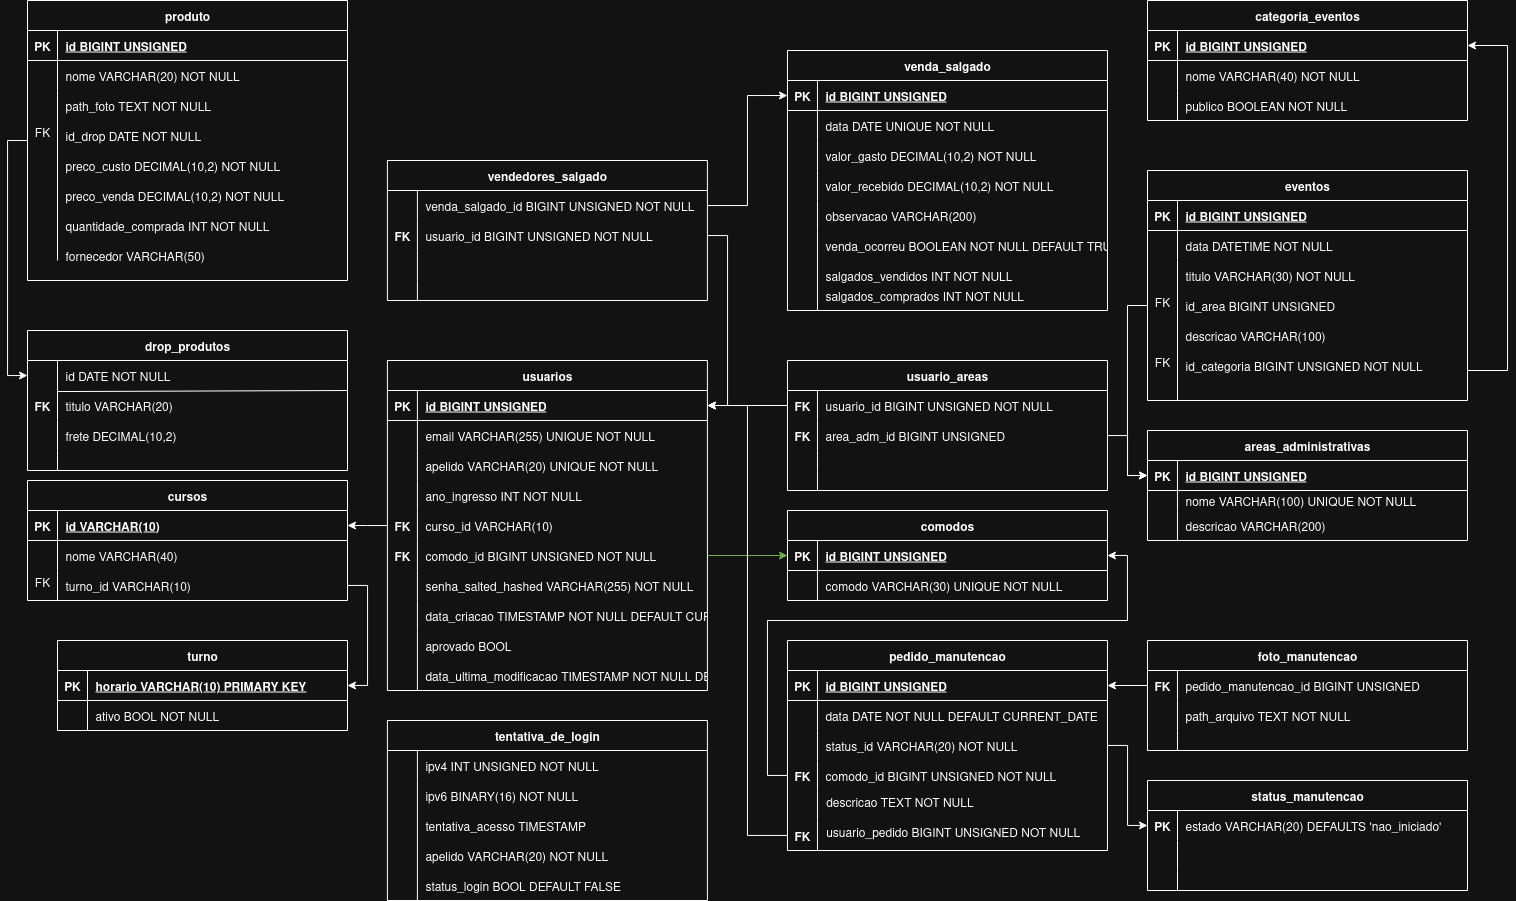
\includegraphics[width=.9\linewidth]{./imgs/Diagrama.png}
\end{center}
\begin{enumerate}
\item Definição do banco de dados
Devemos definir o banco de dados e selecioná-lo para uso. Todas as seguintes definições serão feitas no banco de dados \texttt{diretoria}.
\begin{verbatim}
CREATE DATABASE IF NOT EXISTS diretoria
CHARACTER SET utf8mb4
COLLATE utf8mb4_unicode_ci;

USE diretoria;
\end{verbatim}
\textbf{Turno}:
Define uma tabela que deverá conter os turnos de cursos oferecidos pela UFSCar. Atualmente, estão \texttt{ativos} apenas os turnos noturno e integral, mas a partir de 2026 o curso de Turismo será matutino.
\begin{verbatim}
CREATE TABLE IF NOT EXISTS turno (
        horario VARCHAR(10) PRIMARY KEY,
        esta_ativo BOOLEAN NOT NULL # == TINYINT(1)
);

INSERT INTO turno (horario, esta_ativo) VALUES
        ('noturno', 1),
        ('integral', 1),
        ('vespertino', 0),
        ('matutino', 0);

\end{verbatim}
\textbf{Curso}:
Todo \texttt{curso} está associado a um \texttt{turno} pela chave estrangeira \texttt{turno\_id}. 

\begin{verbatim}
CREATE TABLE IF NOT EXISTS cursos (
        id VARCHAR(10) PRIMARY KEY,
        nome VARCHAR(40) NOT NULL,
        turno_id VARCHAR(10) REFERENCES turno(horario)
);

INSERT INTO cursos (id, nome, turno_id) VALUES
('adm-so', 'bacharelado em administração', 'integral'),
('cc-so ', 'bacharelado em ciência da computação', 'integral'),
('cb-so ', 'bacharelado em biologia', 'integral'),
('cbln-so', 'licenciatura em ciências biológicas', 'integral'),
('cbl-so', 'licenciatura em ciências biológicas', 'integral'),
('cec-so', 'bacharelado em ciências econômicas', 'integral'),
('ep-so ', 'bacharelado em engenharia da produção', 'integral'),
('efl-so', 'bacharelado em engenharia florestal', 'integral'),
('fl-so ', 'licenciatura em fisica', 'integral'),
('gol-so', 'licenciatura em geografia', 'integral'),
('ml-so ', 'licenciatura em matemática', 'integral'),
('pedl-so', 'licenciatura em pedagogia', 'integral'),
('ql-so ', 'licenciatura em química', 'integral'),
('tur-so', 'bacharelado em turismo', 'integral');
\end{verbatim}
\textbf{Comodo}:
Todos os cômodos da casa estarão listados nesta tabela, incluindo um cômodo coringa \texttt{geral}, que indicará manutenções que afetam toda a estrutura da casa. 
\begin{verbatim}
CREATE TABLE IF NOT EXISTS comodos (
        id BIGINT UNSIGNED AUTO_INCREMENT PRIMARY KEY,
        comodo VARCHAR(30) UNIQUE NOT NULL
);  

INSERT INTO comodos(comodo) VALUES
        ('cozinha'),
        ('hall'),
        ('sala de cima'),
        ('quartão'),
        ('varanda do quartão'),
        ('garagem interna'),
        ('garagem externa'),
        ('quintal'),
        ('lavabo'),
        ('corredor'),
        ('suíte master'),
        ('banheiro suíte master'),
        ('closet suíte master'),
        ('suíte bob marley'),
        ('banheiro bob marley'),
        ('suíte placa diretoria'),
        ('banheiro placa diretoria'),
        ('suíte chiqueirinho'),
        ('banheiro suíte chiqueirinho'),
        ('quarto divisória'),
        ('varanda da cozinha'),
        ('quarto da cozinha'),
        ('varanda do quarto da cozinha'),
        ('despensa'),
        ('escada do hall'),
        ('quartinho da escada'),
        ('escada do quintal'),
        ('sala principal'),
        ('quarto cativeiro'),
        ('suíte safadiana'),
        ('banheiro da suíte safadiana'),
        ('varal de baixo'),
        ('varal de cima'),
        ('churrasqueira'),
        ('piscina'),
        ('copa'),
        ('pomar'),
        ('quarto do pomar');
\end{verbatim}
\textbf{Áreas administrativas}:
Haverão múltiplas áreas administrativas, que servirão como 'grupos' de \texttt{usuarios}. O sistema de permissões que controlará a visibilidade de informações em determinadas páginas utilizará as áreas que o \texttt{usuario} pertence para determinar o conteúdo que deve ser mostrado.
\begin{verbatim}
CREATE TABLE IF NOT EXISTS areas_administrativas (
        id BIGINT UNSIGNED AUTO_INCREMENT PRIMARY KEY,
        nome VARCHAR(100) UNIQUE NOT NULL,
        descricao VARCHAR(200)
);

INSERT INTO areas_administrativas (nome, descricao) VALUES
        ('admin', ''),
        ('geral', ''),
        ('marketing', ''),
        ('produtos', ''),
        ('venda salgados', ''),
        ('administrador salgados', ''),
        ('manutenção', '');
\end{verbatim}
\textbf{Usuário}:
Todo \uline{usuario} tem informações associadas a ele, e seu \uline{id} será utilizado por múltiplas tabelas para reunir informações sobre ele de maneiras mais simples. 
\begin{verbatim}
CREATE TABLE IF NOT EXISTS usuarios (
        id BIGINT UNSIGNED AUTO_INCREMENT PRIMARY KEY,
        email VARCHAR(255) UNIQUE NOT NULL,
        apelido VARCHAR(20) UNIQUE NOT NULL,
        ano_ingresso INT NOT NULL,
        curso_id VARCHAR(10) NOT NULL REFERENCES cursos(id),
        comodo_id BIGINT UNSIGNED NOT NULL REFERENCES comodos(id),
        senha_salted_hashed VARCHAR(255) NOT NULL,
        data_criacao TIMESTAMP NOT NULL DEFAULT CURRENT_TIMESTAMP,
        data_ultima_modificacao TIMESTAMP NOT NULL DEFAULT CURRENT_TIMESTAMP ON UPDATE CURRENT_TIMESTAMP
);
INSERT INTO usuarios (email, apelido, ano_ingresso, curso_id, comodo_id, senha_salted_hashed) VALUES
        ('', 'gru', 2023, 'cc-so', 22, '2345678');
\end{verbatim}
\textbf{Usuário Áreas}
A tabela é um tipo-entidade fraco, e associará múltiplos usuários a múltiplas áreas administrativas.
\begin{verbatim}
CREATE TABLE IF NOT EXISTS usuario_areas (

            usuario_id BIGINT UNSIGNED REFERENCES usuarios(id),
         area_adm_id BIGINT UNSIGNED REFERENCES areas_administrativas(id)
);
\end{verbatim}
\textbf{Venda Salgado}
A tabela \texttt{vanda\_salgado} armazenará todos os períodos de vendas e armazenará os valores investido e recebido. Além disso, a quantidade de salgados comprados e vendidos pela entidade.
\begin{verbatim}
CREATE TABLE IF NOT EXISTS venda_salgado (
         id BIGINT UNSIGNED AUTO_INCREMENT PRIMARY KEY,
         data DATE UNIQUE NOT NULL,
         valor_investido DECIMAL(10,2) NOT NULL,
         valor_faturado DECIMAL(10,2) NOT NULL,
         salgados_vendidos INT NOT NULL,
         salgados_comprados INT NOT NULL,
         observacao VARCHAR(200),
         venda_ocorreu BOOLEAN NOT NULL DEFAULT TRUE
);
\end{verbatim}
\textbf{Vendedores Salgado}
Esta tabela é um tipo-entidade fraco, armazenará duas chaves estrangeiras \texttt{venda\_salgado-id}, e \texttt{usuario\_id}. pode haver mais de um vendedor associado a uma venda, e mais de uma venda associada ao mesmo conjunto de usuários, ou conjuntos de usuários diferentes (no caso de uso aplicável, de 1 a 3 responsáveis diariamente).
\begin{verbatim}
CREATE TABLE IF NOT EXISTS vendedores_salgado (
           venda_salgado_id BIGINT UNSIGNED REFERENCES venda_salgado(id),
           usuario_id BIGINT UNSIGNED REFERENCES usuarios(id)
);
\end{verbatim}
\textbf{Categoria Eventos}
A tabela é auxiliar a \texttt{eventos}, e deverá ser uma ferramenta de controle de acesso ao que um \texttt{usuário} poderá visualizar ao acessar a aplicação.
\begin{verbatim}
CREATE TABLE IF NOT EXISTS categoria_eventos (
           id BIGINT UNSIGNED AUTO_INCREMENT PRIMARY KEY,
           nome VARCHAR(40) NOT NULL,
           publico BOOLEAN NOT NULL
);
\end{verbatim}
\textbf{Eventos}
A tabela \texttt{eventos} será generalista. Isso significa que os eventos associados a ela também terão áreas específicas. A princípio, implementaremos apenas os eventos da área \texttt{geral}, e posteriormente visões diferentes associadas ao grupo de usuários pertinente. Estes dados serão a base para a construção de um front-end de calendário interativo, onde os usuários poderão adicionar, visualizar e editar eventos.
\begin{verbatim}
CREATE TABLE IF NOT EXISTS eventos (
           id BIGINT UNSIGNED AUTO_INCREMENT PRIMARY KEY,
           data_hora DATETIME NOT NULL,
           titulo VARCHAR(30) NOT NULL,
           id_area BIGINT UNSIGNED REFERENCES areas_administrativas(id),
           descricao VARCHAR(100),
           id_categoria BIGINT UNSIGNED REFERENCES categoria_eventos(id)
);
\end{verbatim}
\textbf{Drop Produtos}
Esta tabela será a referência para todo \texttt{produto} que for lançado na mesma ocasião, por exemplo, um modelo de caneca, tirante, colete, samba, doll e saia lançados e vendidos em conjunto para o TUSCA.
\begin{verbatim}
CREATE TABLE IF NOT EXISTS drop_produtos (
           id DATE PRIMARY KEY,
           titulo VARCHAR(40) NOT NULL,
           valor_frete DECIMAL(10,2) NOT NULL
);
\end{verbatim}
\textbf{Produto}
A tabela armazenará diferentes modelos de produtos desenvolvidos e vendidos pela República. Os valores incluem preços, caminho da foto, um identificador de \texttt{drop\_produtos}, e a quantidade que a República comprou.
\begin{verbatim}
CREATE TABLE IF NOT EXISTS produto (
           id BIGINT UNSIGNED AUTO_INCREMENT PRIMARY KEY,
           id_drop DATE REFERENCES drop_produtos(id),
           custo_frete DECIMAL(10,2)

);
\end{verbatim}
\end{enumerate}
\item 4.2.6 style
\label{sec:org31fec0a}
O diretório \texttt{style} centraliza todos os arquivos que definem a aparência visual do sistema, incluindo cores, fontes, layouts e mais. Neste, haverá principalmente arquivos \texttt{css} e outros estilizadores para os elementos da interface.
\end{enumerate}
\end{document}
